\chapter{Introduction}
\label{chap:introduction}
Since 1979, the areal extent of Arctic sea ice in early autumn has shrunk by 80\% according to satellite data~\citep{NSIDC}. According to new satellite data sets, the decline appears to be particularly rapid after 2000~\citep{Wu2012}. The dramatic reduction in sea ice extent may have contributed strongly to the rapid warming of the Arctic, due to increases in latent and sensible heat fluxes from the ocean~\citep{Screen2010}, and due to the sea-ice-albedo effect (@cite someone). The rapid warming of the Arctic compared to the global mean has become known as "Arctic amplification"~\citep{Graversen2008}, but the reasons for this amplification are not fully understood.

Globally, low clouds have a net cooling effect reflecting solar radiation, due to their high albedo. Clouds also absorb and emit terrestrial longwave radiation which has a warming effect at the surface. In the Arctic the solar radiation is less than at lower latitudes, and the warming effect of downwelling longwave radiation overpowers the cooling effect of reflecting shortwave radiation, since there is less to reflect, thus low clouds have a net warming effect in the Arctic~\citep{Shupe2004}. The Arctic cloud cover~\citep{Curry1996} is dominated by low layered clouds (stratus), and so the climate effect of low clouds in the Arctic is important to study.

Decreasing sea ice extent could lead to an increase in the aerosol number concentrations in the area where ice has retreated. The open sea surface itself would lead to an increase in release of sea salt and DMS (dimethyl sulfide) to the lower atmosphere. The lack of sea ice would also increase the likelihood that the sea could be used for shipping, which would further increase the aerosol number concentration.

The enhancement of evaporation from the ocean with diminishing sea ice and the increase in aerosol number concentration from open water and shipping could lead to denser and longer-lived low clouds in the area of sea ice retreat (@cite someone). The  hypothesis of this thesis is that these clouds would then have a different radiative effect, and by that influence the further retreat of sea ice.


%\textbf{Must rewrite: Aside from producing precipitation, clouds have a profound effect on our climate. If you consider the overall effect of all clouds on the surface temperature, they have a cooling effect because they block incoming solar radiation. However, the effect of an individual cloud depends on many factors such as its height, thickness, location, and whether it is day or night. .... tatt fra nettet, Colorado State, CMMAP}.

\section{Main goal}
Studies by~\citet{Eastman2010b} using visual cloud reports from the Arctic, with surface and satellite observations, and by~\citet{Kay2009} and~\citet{Palm2010} using lidar and radar observations have confirmed that the low-cloud amount over the Arctic oceans varies inversely with sea ice amount. This means that there is an increase in cloud amount when there is less sea ice. In this thesis I will study if these clouds are also denser and more persistent, and could lead to an enhanced warming and reduced sea ice amount, also known as a positive feedback.

The effect of increase in aerosol concentrations from shipping and open water, and the effect of enhanced evaporation from open water are studied separately and combined. The main goal is to find whether more open ocean and/or larger aerosol loads will lead to changes in clouds that could enhance downwelling longwave radiation and decrease upwelling shortwave radiation, both of which have a warming effect at the surface, and therefore have a positive feedback enhancing warming of the Arctic.

%(Something citing the IPCC report 2013 on the ice conditions in the Arctic, and something about Arctic clouds and radiation?)

The findings in my thesis have been achieved by use of the Advanced Research Weather, Research and Forecasting (ARW) model, with some of the most recently developed code (by Greg Thompson~\citep{Thompson2014}) for cloud micro physics and aerosols and their effects on radiation.% The results build further on the work of other researchers @name-some-and-cite and may raise some questions for further research within the field.

\section{Area description}
The study area is in the Arctic and covers the Beaufort Sea and small parts of Alaska and Canada (figure~\ref{fig:area}). (@ input Alaska and Canada on the map!)

\begin{figure}
\centering
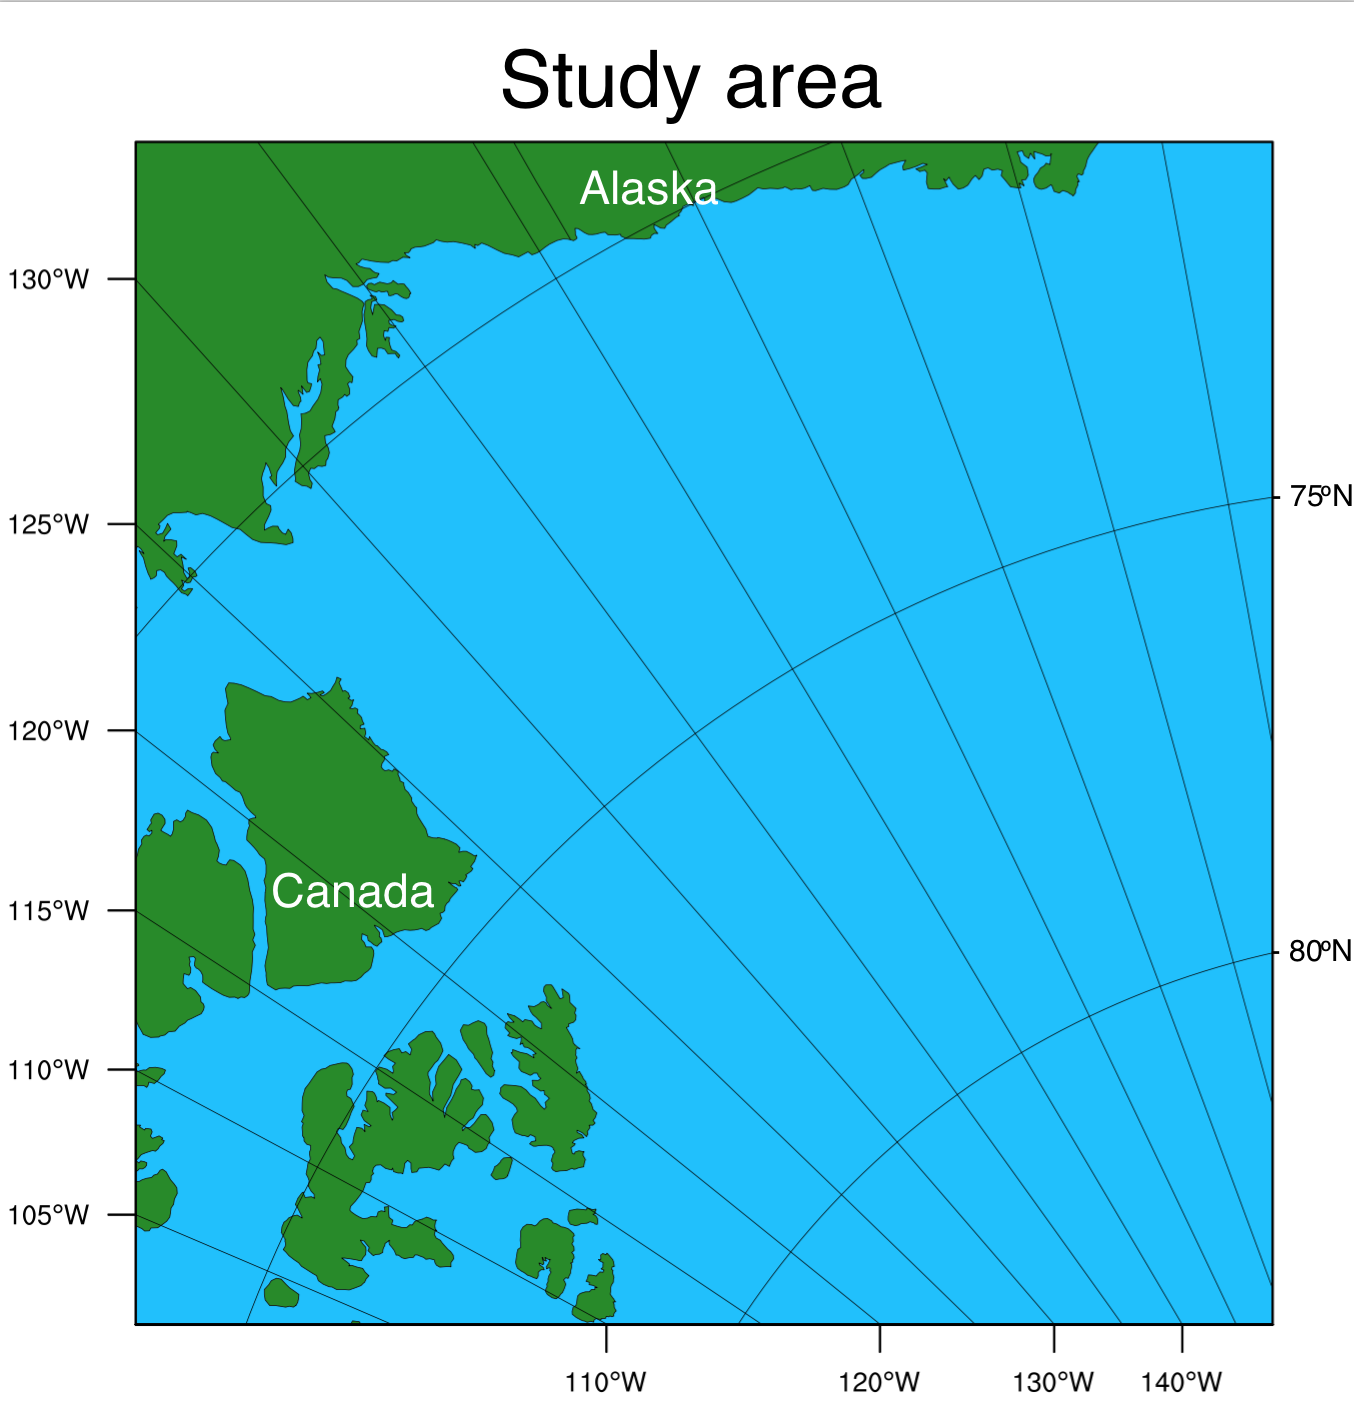
\includegraphics[width=0.7\textwidth]{introduction/studyarea.png}
\caption{An overview of the study area. The bottom right corner is the northernmost point and the y-axes show longitude and latitude to the left and right, respectively.}
\label{fig:area}
\end{figure}
 
There are a few reasons for choosing this as the study area. First it is in the Arctic, and sea ice is present there in autumn, even in 2012 when there was record low sea ice extent (eg. National Snow and Ice Data Center~\citep{NSIDC}). Also it has been subject to field campaigns: Surface Heat Budget of the Arctic Ocean (SHEBA)~\citep{Uttal2002}, First International Satellite Cloud Climatology Project Regional Experiment Arctic cloud Experiment (FIRE ACE)~\citep{Curry2000}, Mixed-Phase Arctic Cloud Experiment (M-PACE)~\citep{Verlinde2007} and more. There are a few studies on Arctic clouds that include this area and data from some of the aforementioned field campaigns. These provide parts of the science basis for my study and selection of literature and studies for comparison and questions. Quite a few studies are based on satellite data analysis, and some of these are mentioned in the next section as background and motivation for my thesis.

\section{Background}%Background and motivation?
\label{sec:background}
%Some new (and older) research that makes my thesis interesting and relevant to the field. No one has done this study with a weather forecasting model, it is interesting to look at changes in parameters in similar meteorological conditions, the same initial and boundary conditions in every run.
%Describe some of the work done by %\citet{Palm2010, Wu2012} and others on autumn low clouds in the Arctic to emphasize the importance of my work.

A study by~\citet{Schweiger2008} investigated the connection between sea ice variability and cloud cover over over the Arctic seas during autumn. They analysed the ERA-40 re-analysis products and some satellite data sets. %the Television and Infrared Observation Satellite (TIROS) Operational Vertical Sounder (TOVS) Polar Pathfonder datasets~\citep{Schweiger2008}.
They found that that sea ice retreat was linked to a decrease in low-level (surface to $\sim$1.9~km) cloud amount and an increase in mid-level ($\sim$1.9 to 6.1~km) clouds. They state that the decrease in static stability and deepening of the atmospheric boundary layer, following ice retreat, contribute to the rise in cloud level. 
 %the 40-yr European Centre for Medium-Range Weather Forecasts (ECMWF) Re-Analysis (ERA-40) products

\citet{Vavrus2010} investigated the behaviour of clouds, during intervals of rapid sea ice loss in the Arctic in the 21st century. The study was done by use of the Community Climate System Model (CCSM3). They conclude that cloud changes accelerate rapid loss of sea ice in autumn. @\textit{nevne hvilke skyendringer dette er} %Their results support that cloud changes appear to accelerate rapid loss of sea ice in autumn, and possibly in winter. They also conclude that "the trends in total cloudiness during rapid ice loss events are explained almost entirely by low-level clouds" and that "a positive feedback from primarily low cloud changes amid a warming climate".

\citet{Kay2009} combined satellite data sets and complementary atmosphere reanalysis data to study the Arctic cloud and atmospheric structure during summer and early Autumn over the years 2006-2008. This covers the (at the time) record low sea ice extent from 2007. In contrast to the study by~\citet{Schweiger2008} they found more low-level cloud. The re-analysis used in~\citet{Schweiger2008} was for the time period 1964-2001, which is not the same period as~\citet{Kay2009} studied. (@\textit{finn kritikk av ERA-40, hvorfor er ikke S08 til å stole på..})

\citet{Eastman2010a} analyzed visual cloud reports from the Arctic for year-to-year variations and found that following a low-ice September there would be enhanced low cloud cover. @\textit{når? senere i sesongen? hele vinteren? sjekk!}

A study by~\citet{Palm2010} using satellite and lidar data  found that areas of open water were associated with greater polar cloud fraction. %from the Ice Cloud, and Land Elevation Satellite (ICESat) and the Cloud-Aerosol Lidar and Infrared Pathfinder Satellite Observation (CALIPSO)  found that areas of open water were associated with greater polar cloud fraction.

A common uncertainty and missing link in a few of these studies is that they did not look at liquid water content, effective radii and other parameters affecting the radiative properties of the clouds. In this study, that is what I want to look in to, how these properties are influenced by the changing sea ice, and if changes in the clouds enhance the sea ice melt.

%--------- Introduction based on master description ---------
%Since 1979, the areal extent of Arctic sea ice in early autumn has shrunk by 80\%, according to satellite data (e.g. National Snow and Ice Data Center, U.S.A.). The decline appears to be particularly rapid after 2000, as documented by new satellite data sets (Wu and Lee, 2012). The dramatic reduction in sea ice extent may have contributed strongly to the rapid warming of the Arctic observed in recent years, due to increased fluxes of sensible and latent heat from the Arctic Ocean to the overlying atmosphere (Screen and Simmonds, 2010). Other factors may also contribute such as changes in the atmospheric circulation or cloud changes. In particular, it has been suggested that the enhanced evaporation from the ice-free ocean may lead to more persistent and denser clouds. Satellite retrievals suggest that in the autumn the Arctic stratus clouds have indeed become more dense and extensive over the last 10 years, or so (Palm et al., 2010). It is well known that in the Arctic the low clouds have a warming effect on the surface due to their enhancement of downwelling radiation (Intrieri et al., 2002). Therefore, one can envisage a positive feedback between shrinking sea ice (due to global warming), enhanced evaporation, increased effective cloud cover, enhanced downwelling longwave radiation and warming surface temperatures. However, such a feedback loop has not been established, and it can not be ruled out that the positive correlation observed over only a few years between sea ice extent and cloud amount may be a co-incidence. Furthermore, cloud properties may also change due to aerosol changes, e.g., due to increasing emissions of SO2 from ship traffic, as well as di-methyl- sulfide (DMS), sea salt and primary organic matter from the open ocean. Such aerosol changes may render the clouds optically thicker (Lubin and Vogelmann, 2006), with a possible additional positive feedback loop.


%Is my work new thinking and does it seem to be very extensive?

%Should this whole chapter be a part of introduction..?

%Previous studies, shed light on why my study is interesting and may be of importance.

%Palm, Kay and Gettleman, Eastman and Warren according to the IPCC report!

\section{Structure of the thesis}
%In the following chapter~\ref{chap:background} I will present the background for my thesis; what work I hope to compare my results to and relate my thesis to. Also I will touch upon why the subject of my thesis is important. 
In the following chapter, Chapter~\ref{chap:theory}, the most important theory needed to understand some of the processes in clouds and their possible effect on the sea ice is presented. Chapter~\ref{chap:modmet} is where I explain which model and tools I have used and how I have worked with them to get the results presented and discussed in Chapter~\ref{chap:results}. A summary of main findings and conclusions are presented in the last chapter, Chapter~\ref{chap:summaryconclusions}.